% Author: Dominik Harmim <xharmi00@stud.fit.vutbr.cz>
% Author: Vojtěch Hertl <xhertl04@stud.fit.vutbr.cz>

\documentclass[a4paper, 11pt]{article}


\usepackage[czech]{babel}
\usepackage[utf8]{inputenc}
\usepackage[left=2cm, top=3cm, text={17cm, 24cm}]{geometry}
\usepackage{times}
\usepackage{verbatim}
\usepackage{enumitem}
\usepackage{graphicx} % vkládání obrázků
\usepackage[unicode]{hyperref}
\hypersetup{
	colorlinks = true,
	hypertexnames = false,
	citecolor = red
}


\newcommand{\RNum}[1]{\uppercase\expandafter{\romannumeral #1\relax}} % makro na sázení římských čísel


\begin{document}


	%%%%%%%%%%%%%%%%%%%%%%%%%%%%%%%% Titulní stránka %%%%%%%%%%%%%%%%%%%%%%%%%%%%%%%%
	\begin{titlepage}
		\begin{center}
			
\includegraphics[width=0.77\linewidth]{inc/FIT_logo.pdf} \\

			\vspace{\stretch{0.382}}

			\Huge{Projektová dokumentace} \\
			\LARGE{\textbf{TODO }} \\
			\Large{Tým ModelX, varianta 2: Doprava zboží nebo osob}
			\vspace{\stretch{0.618}}
		\end{center}

		\begin{minipage}{0.4 \textwidth}
			{\Large \today}
		\end{minipage}
		\hfill
		\begin{minipage}[r]{0.6 \textwidth}
			\Large
			\begin{tabular}{l l l}
				& \textbf{Dominik Harmim} & \textbf{(xharmi00)} \\
				& Vojtěch Hertl & (xhertl04) \\
			\end{tabular}
		\end{minipage}
	\end{titlepage}



	%%%%%%%%%%%%%%%%%%%%%%%%%%%%%%%% Obsah %%%%%%%%%%%%%%%%%%%%%%%%%%%%%%%%
	\pagenumbering{roman}
	\setcounter{page}{1}
	\tableofcontents
	\clearpage



	%%%%%%%%%%%%%%%%%%%%%%%%%%%%%%%% Úvod %%%%%%%%%%%%%%%%%%%%%%%%%%%%%%%%
	\pagenumbering{arabic}
	\setcounter{page}{1}

	\section{Úvod}

	V této práci je řešen proces sestavování modelu[citace] pro rozvoz jídla po Brně firmou FreshBox[citace] a jeho následná simulace[citace]. Díky tomuto modelu a simulačním experimentům nad ním bude možno pozorovat efektivitu a přínos v různých podmínkách. Smyslem experimentů je zjistit, zda by se změnou některého z faktorů mohl systém zdokonalit.



	\subsection{Autoři, zdroje}

	Projekt vypracovali studenti Dominik Harmim a Vojtěch Hertl z VUT v Brně, FIT. Při řešení této práce bylo využito zdrojů z předmětu Modelování a simulace.

	\subsection{Ověření validity}

	Ověřování validity probíhalo telefonicky a elektronicky s vedoucí firmy FreshBox, Mgr. Silvií Obadalovou (obadalova@freshbox.cz). Na základě této komunikace byla získána všechna data potřebná k experimentálnímu ověřování validity modelu. Validita byla také ověřena pomocí experimentů.
	\clearpage


	%%%%%%%%%%%%%%%%%%%%%%%%%%%%%%%% Rozbor tématu a použitých metod/technologií %%%%%%%%%%%%%%%%%%%%%%%%%%%%%%%%
	\section{Rozbor tématu a použitých metod/technologií}

	Všechna data jsou zprůměrována z dostupných informací od paní magistry Obadalové, vedoucí firmy. \\

	Zákazníci mají předem objednaná jidla od firmy FreshBox, která tato jídla každý den od 6:30 hod. do 12:30 hod. rozváží zákazníkům po Brně a okolí. Firma FreshBox rozváží jidlo A auty, přičemž jedno auto je schopné naložit maximálně B jídel. Každý den se rozváží průměrně C jídel. Firma má na začátku rozvozu již všechna jídla připravena a v 6:30 se připraví všechna auta, do kterých se naloží maximální počet jídel, který je dán kapacitou auta. Naložení jednoho auta průměrně trvá D minut. Rozvoz všech jídel jednoho auta trvá průměrně E minut. Při tomto rozvozu každé auto urazí průměrně F km. Pro rozvoz se požívají auta značky G. Tato auta mají spotřebu H l/100km banzínu/nafty. Když auto rozveze všechna naložená jídla, vrátí se na pobočku FreshBox, aby se mohla naložit další jídla. Tento proces se opakuje tak dlouho, dokud buď nejsou rozvezena všechna jídla, nebo dokud neskončí pracovní směna. Jeden zákazník (právnická nebo fyzická osoba) si samozřejmě může objednat více jídel na jedno místo doručení. Průměrná hodnota objednávky jednoho zákazníka v jeden den činí I Kč.

	\subsection{Použité postupy}

	Pro vytvoření modelu byl použit programovací jazyk C++ za podpory simulační knihovny SIMLIB [citace]. Tyto technologie jsou ideální pro řešení zadaného problému, jelikož poskytují všechna potřebná rozhraní k implementaci modelu. Dále byly použity postupy popsané v prezentaci k předmětu IMS k vytváření Petriho sítě[citace] a samotnému programování za použití knihovny SIMLIB[citace].

	\subsection{Popis původu použitých metod/technologií}

	TODO vyjmenovat všechny technologie a autory u nich, např. Knihovna SIMLIB ve verzi ..., autor Dr. Ing. Petr Peringer.


	%%%%%%%%%%%%%%%%%%%%%%%%%%%%%%%% Koncepce modelu %%%%%%%%%%%%%%%%%%%%%%%%%%%%%%%%
	\section{Koncepce modelu}



	%%%%%%%%%%%%%%%%%%%%%%%%%%%%%%%% Architektura simulačního modelu %%%%%%%%%%%%%%%%%%%%%%%%%%%%%%%%
	\section{Architektura simulačního modelu}



	%%%%%%%%%%%%%%%%%%%%%%%%%%%%%%%% Podstata simulačních experimentů a jejich průběh %%%%%%%%%%%%%%%%%%%%%%%%%%%%%%%%
	\section{Podstata simulačních experimentů a jejich průběh}




	%%%%%%%%%%%%%%%%%%%%%%%%%%%%%%%% Shrnutí simulačních experimentů a závěr %%%%%%%%%%%%%%%%%%%%%%%%%%%%%%%%
	\section{Shrnutí simulačních experimentů a závěr}



	%%%%%%%%%%%%%%%%%%%%%%%%%%%%%%%% Citace %%%%%%%%%%%%%%%%%%%%%%%%%%%%%%%%
	\clearpage
	\bibliographystyle{czechiso}
	\renewcommand{\refname}{Literatura}
	\bibliography{dokumentace}



	%%%%%%%%%%%%%%%%%%%%%%%%%%%%%%%% Přílohy %%%%%%%%%%%%%%%%%%%%%%%%%%%%%%%%
	\clearpage
	\appendix

	\section{Petriho síť}
	\begin{figure}[!ht]
		\centering
		\vspace{-1.2cm}
		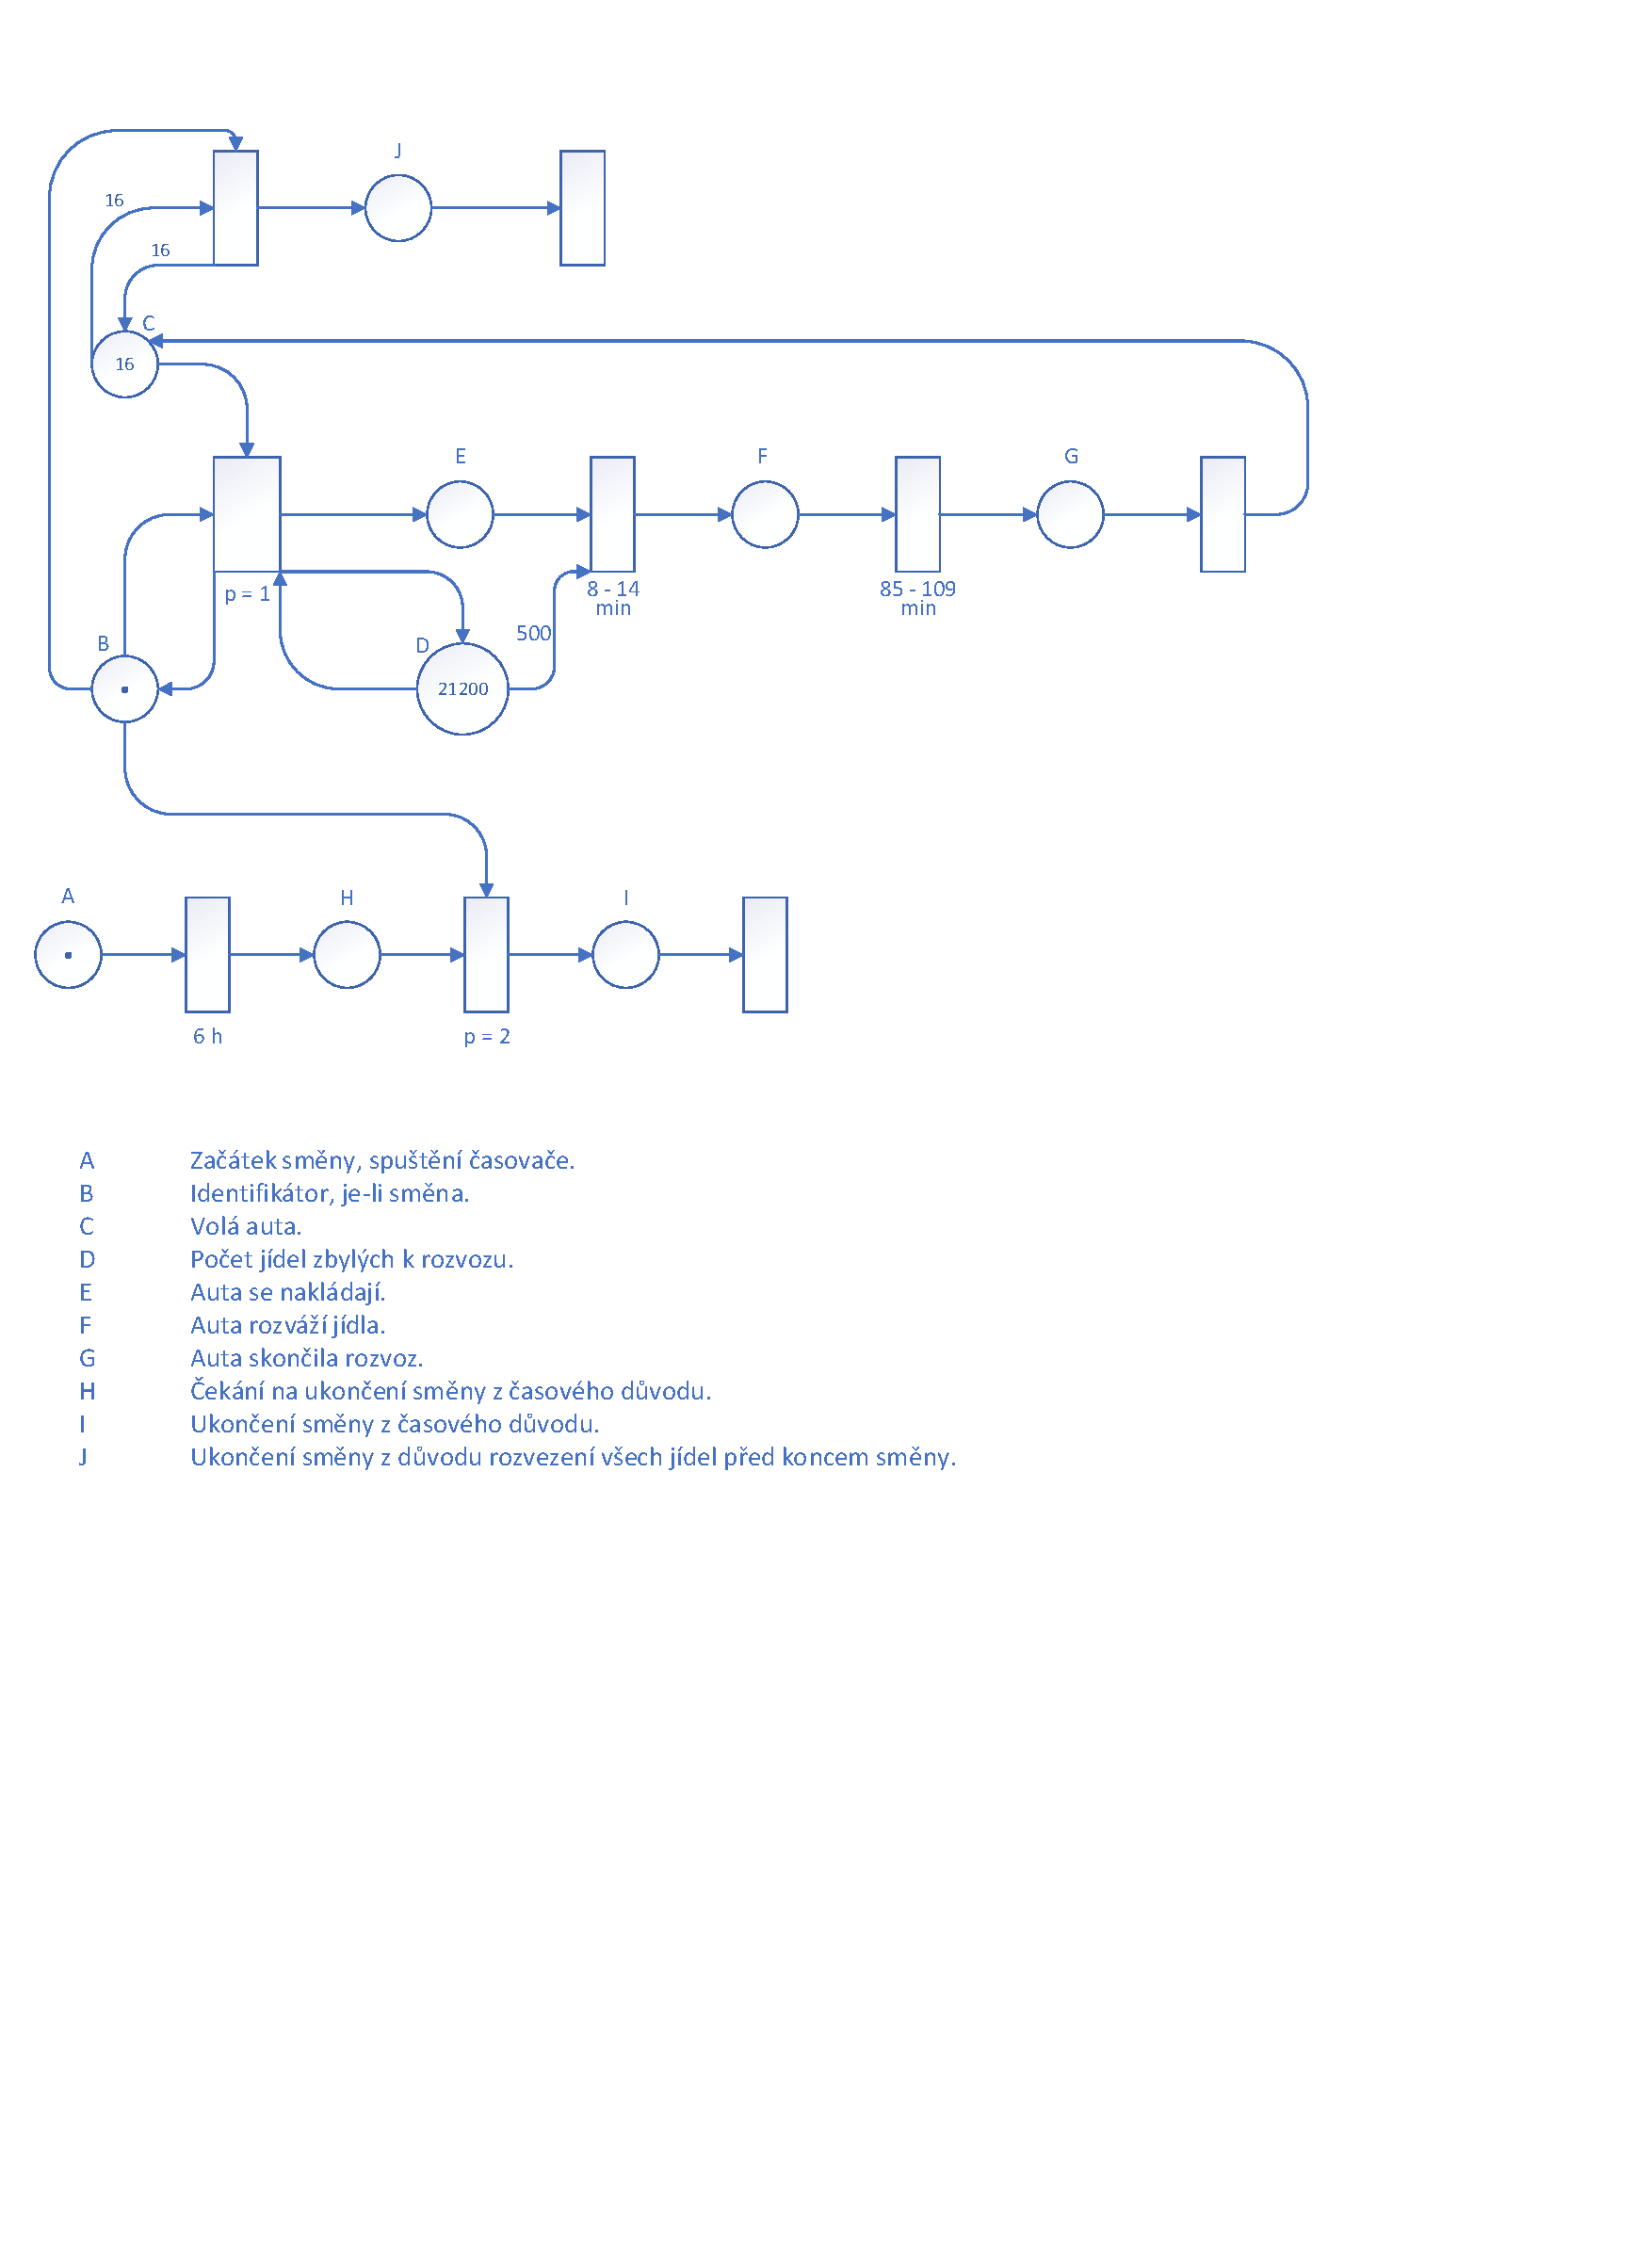
\includegraphics[width=0.95\linewidth]{inc/petri_net.pdf}
		\caption{Petriho síť}
		\label{figure:petri_net}
	\end{figure}



\end{document}